% You can choose whether you prefer a single or double column appendix.
% Whatever you choose, you will need to stick to it throughout the appendix.
% For double column style, comment the next line.
\onecolumn

\appendix
\begin{appendices}

\section{Posterior Plots}
\label{sec:apx:posterior_plots}

\begin{figure}[htb]
  \centering
  \includegraphics[width=0.835\linewidth]{media/images/Posteriors_UNet_original_half_round_8.png}
  \caption{Comparison between U-Net (blue) and U-Net with half the number of simulations (red) after 8 rounds of TMNRE. The dotted line shows the ground-truth value.}
  \label{fig:posterior_unet_half}
  \Description[<short description>]{<long description>}
\end{figure}

\begin{figure}[htb]
  \centering
  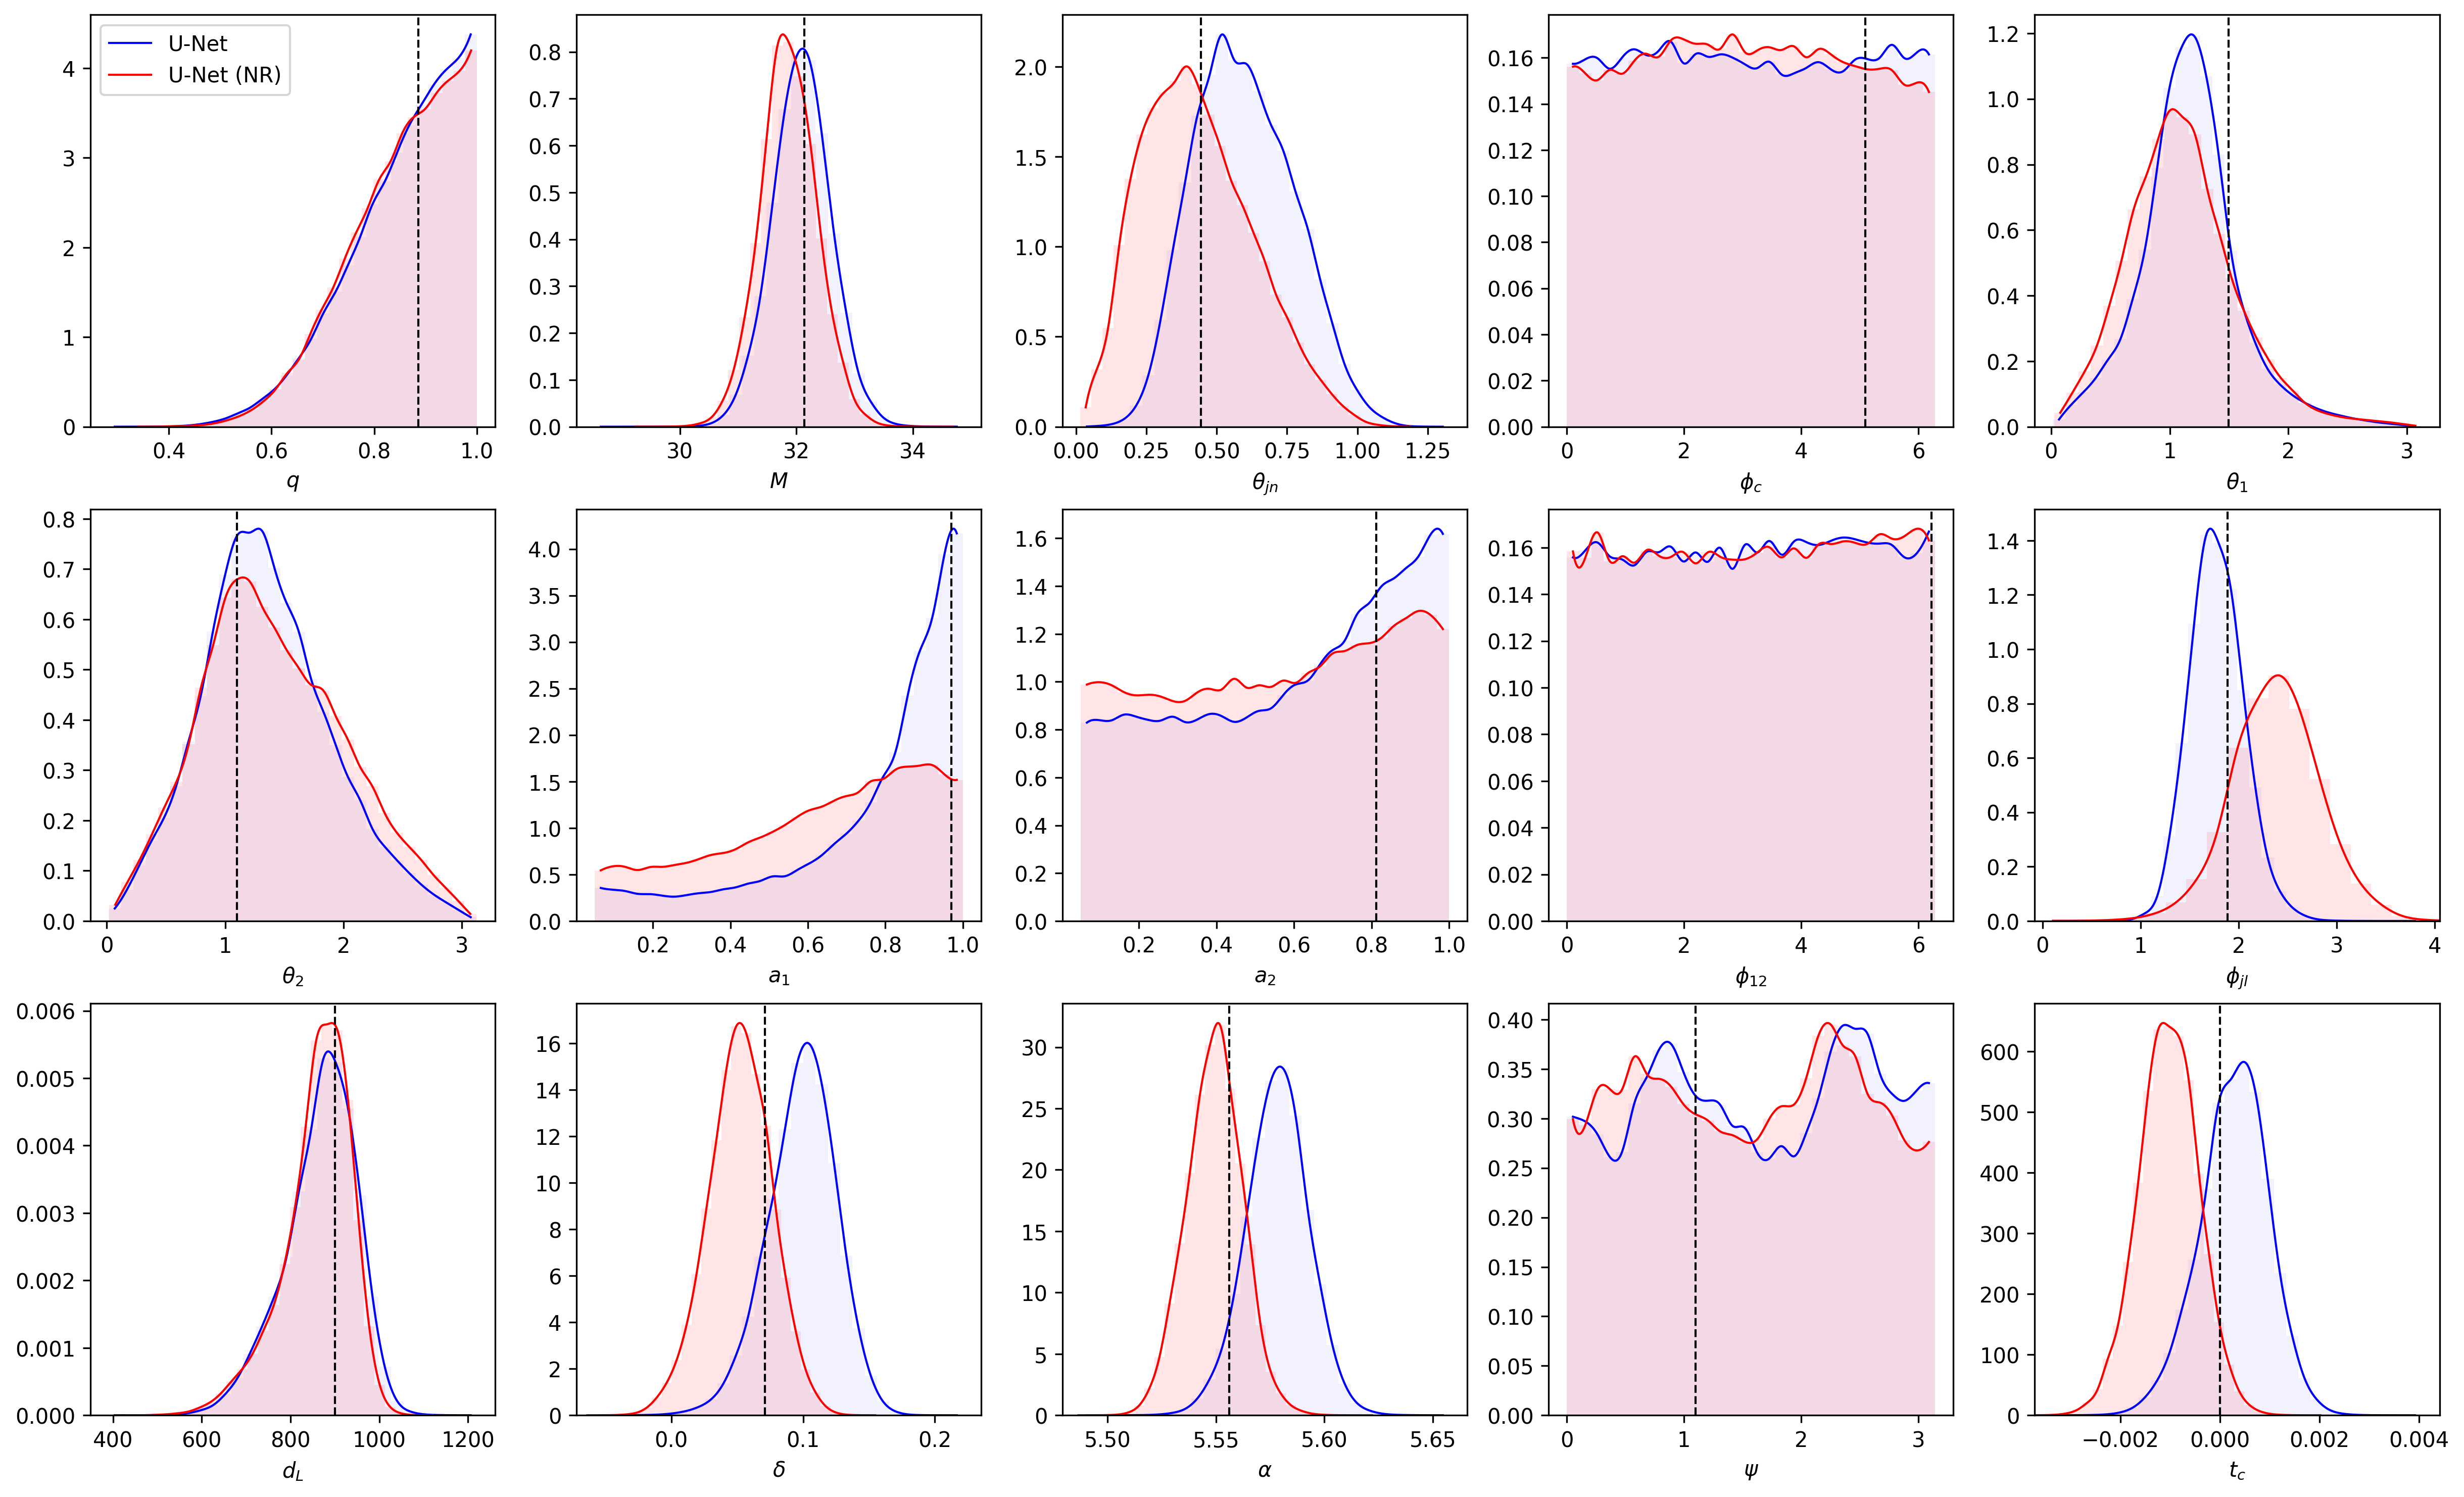
\includegraphics[width=0.835\linewidth]{media/images/Posteriors_UNet_NoReinit_round_8.png}
  \caption{Comparison between U-Net (blue) and U-Net with no re-initialisation (red) after 8 rounds of TMNRE.}
  \label{fig:posterior_unet_noreinit}
  \Description[<short description>]{<long description>}
\end{figure}

\begin{figure}[htb]
  \centering
  \includegraphics[width=0.85\linewidth]{media/images/Posteriors_AttentionUNet_2_round_8.png}
  \caption{Comparison between U-Net (blue) and Attention U-Net (red) after 8 rounds of TMNRE. The dotted line shows the ground-truth value.}
  \label{fig:posterior_attention_unet}
  \Description[<short description>]{<long description>}
\end{figure}

\begin{figure}[htb]
  \centering
  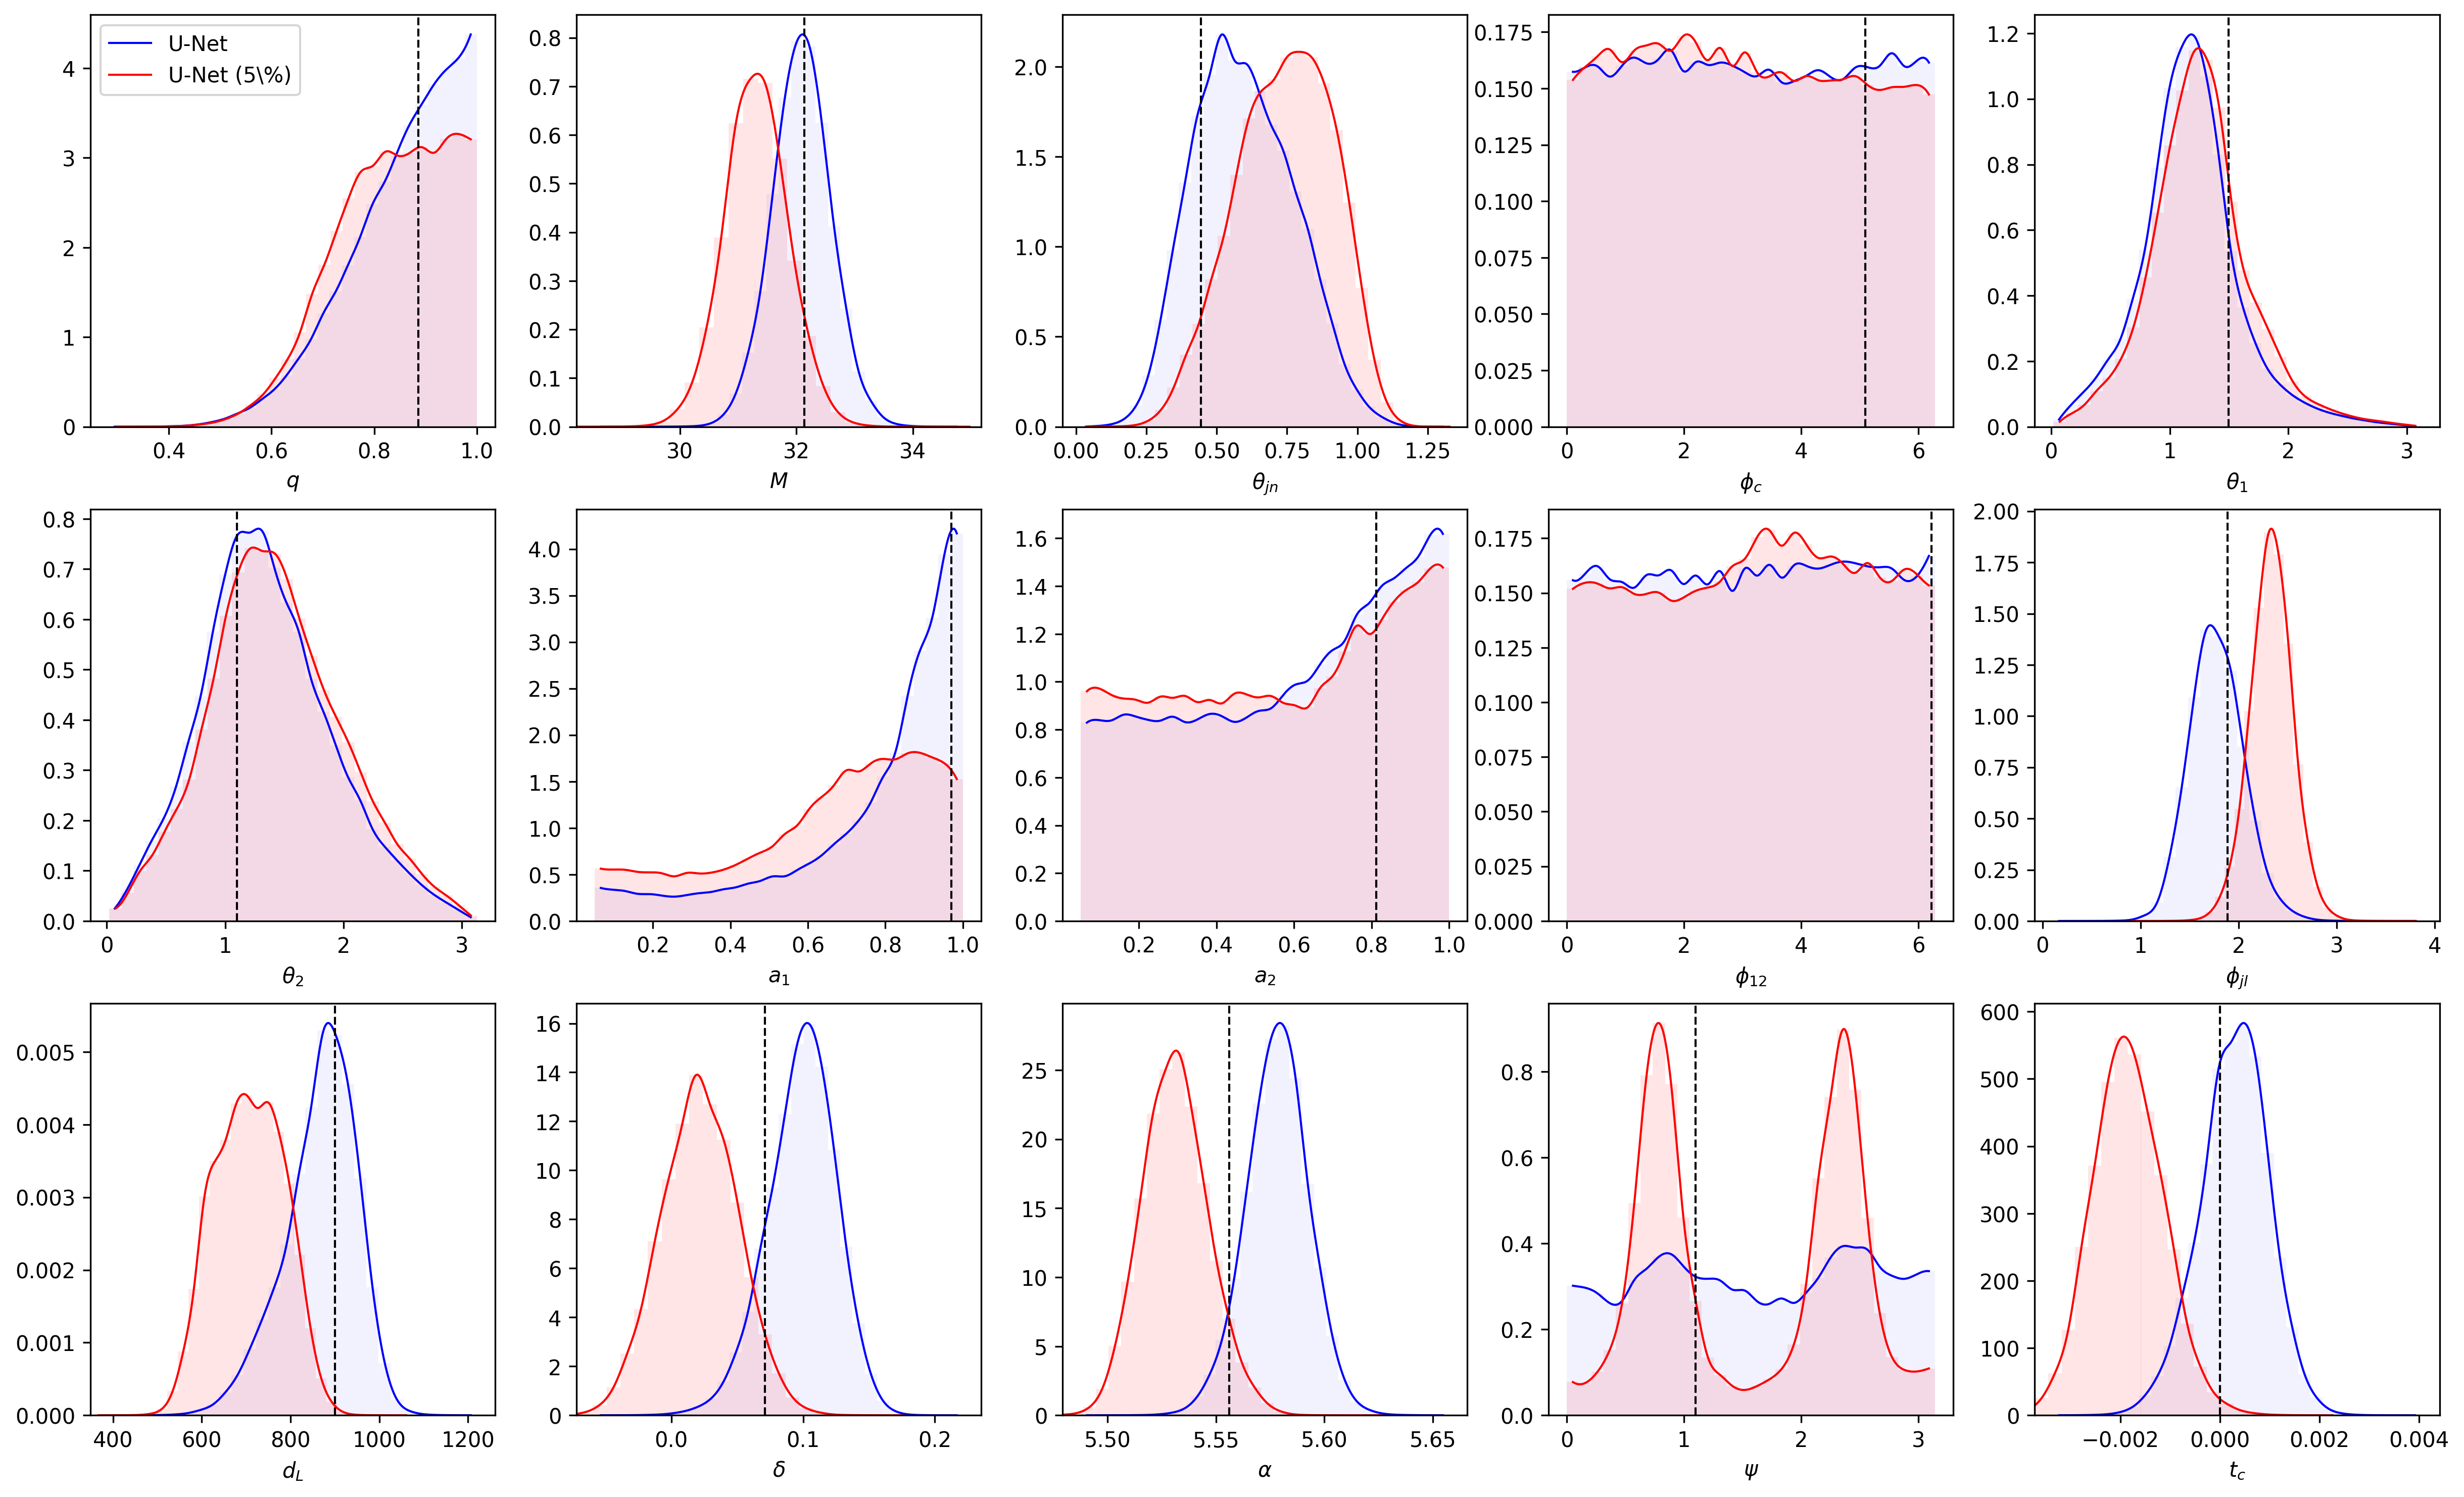
\includegraphics[width=0.85\linewidth]{media/images/Posteriors_UNet_pruned5_2_round_8.png}
  \caption{Comparison between U-Net (blue) and U-Net 5\% pruned (red) after 8 rounds of TMNRE. The dotted line shows the ground-truth value.}
  \label{fig:posterior_unet_pruned_5pc}
  \Description[<short description>]{<long description>}
\end{figure}

\begin{figure}[htb]
  \centering
  \includegraphics[width=0.85\linewidth]{media/images/Posteriors_UNet_pruned10_round_8.png}
  \caption{Comparison between U-Net (blue) and U-Net 10\% pruned (red) after 8 rounds of TMNRE. The dotted line shows the ground-truth value.}
  \label{fig:posterior_unet_pruned_10pc}
  \Description[<short description>]{<long description>}
\end{figure}

\begin{figure}[htb]
  \centering
  \includegraphics[width=0.85\linewidth]{media/images/Posteriors_ViT_pretrained_2_round_3.png}
  \caption{Comparison between U-Net (blue) and ViT transformer (red) after 3 rounds of TMNRE. The dotted line shows the ground-truth value.}
  \label{fig:posterior_vit}
  \Description[<short description>]{<long description>}
\end{figure}

\FloatBarrier

\section{U-Net Architecture}
\label{sec:apx:u-net_architecture}

\begin{figure}[htb]
	\centering
	\begin{tikzpicture}[node distance=1.0cm]
		
    %%% NODES
    
    \node (input) [input, label=west:\tiny 8192$\times$3, text width=2cm] {\small Input wave, $d(t)+n(t)$};

    \node (conv1) [conv, below of=input, label=west:\tiny 8192$\times$16] {\small 3$\times$1 conv, 16};
    \node (conv2) [conv, below of=conv1, label=west:\tiny 8192$\times$16] {\small 3$\times$1 conv, 16};
    
    \node (pool1) [pool, below of=conv2, label=west:\tiny 1024$\times$16] {\small max pool, /8};
    
    \node (conv3) [conv, below of=pool1, label=west:\tiny 1024$\times$32] {\small 3$\times$1 conv, 32};
    \node (conv4) [conv, below of=conv3, label=west:\tiny 1024$\times$32] {\small 3$\times$1 conv, 32};
    
    \node (pool2) [pool, below of=conv4, label=west:\tiny 128$\times$32] {\small max pool, /8};
    
    \node (conv5) [conv, below of=pool2, label=west:\tiny 128$\times$64] {\small 3$\times$1 conv, 64};
    \node (conv6) [conv, below of=conv5, label=west:\tiny 128$\times$64] {\small 3$\times$1 conv, 64};
    
    \node (pool3) [pool, below of=conv6, label=west:\tiny 16$\times$64] {\small max pool, /8};
    
    \node (conv7) [conv, below of=pool3, label=west:\tiny 16$\times$128] {\small 3$\times$1 conv, 128};
    \node (conv8) [conv, below of=conv7, label=west:\tiny 16$\times$128] {\small 3$\times$1 conv, 128};
    
    \node (pool4) [pool, below of=conv8, label=west:\tiny 2$\times$128] {\small max pool, /8};

    \node (conv9) [conv, below of=pool4, label=west:\tiny 2$\times$256] {\small 3$\times$1 conv, 256};
    \node (conv10) [conv, below of=conv9, label=west:\tiny 2$\times$256] {\small 3$\times$1 conv, 256};
    
    %%%%%
    
    \node (upconv1) [upconv, right of=conv10, label=east:\tiny 2$\times$128, xshift=3.5cm] {\small 3$\times$1 upconv, 128};
    \node (zp1) [concat, above of=upconv1, label=east:\tiny 16$\times$128, yshift=-0.49cm] {\small zero-padding \hspace{0.4cm} };
    \node (concat1) [concat, above of=zp1, label=east:\tiny 32$\times$128, yshift=-0.3cm] {\small concatenation \hspace{0.25cm} };
    \node (upconvrelu1) [convx2, text width=3cm, above of=concat1, label=east:\small \hspace{-0.25cm} $\times$2 \tiny 16$\times$128] {\small 3$\times$1 conv, 128, stride 2 + ReLU};
    
    \node (AG1) [AG, left of=concat1, xshift=-1.5cm] {\footnotesize $\sim$};

    \node (upconv2) [upconv, above of=upconvrelu1, label=east:\tiny 16$\times$64] {\small 3$\times$1 upconv, 64};
    \node (zp2) [concat, above of=upconv2, label=east:\tiny 128$\times$64, yshift=-0.49cm] {\small zero-padding \hspace{0.25cm} };
    \node (concat2) [concat, above of=zp2, label=east:\tiny 256$\times$64, yshift=-0.3cm] {\small concatenation \hspace{0.25cm} };
    \node (upconvrelu2) [convx2, text width=3cm, above of=concat2, label=east:\small \hspace{-0.25cm} $\times$2 \tiny 128$\times$64] {\small 3$\times$1 conv, 64, stride 2 + ReLU};
    
    \node (AG2) [AG, left of=concat2, xshift=-1.5cm] {\footnotesize $\sim$};

    \node (upconv3) [upconv, above of=upconvrelu2, label=east:\tiny 128$\times$32] {\small 3$\times$1 upconv, 32};
    \node (zp3) [concat, above of=upconv3, label=east:\tiny 1024$\times$32, yshift=-0.49cm] {\small zero-padding \hspace{0.25cm} };
    \node (concat3) [concat, above of=zp3, label=east:\tiny 2048$\times$32, yshift=-0.3cm] {\small concatenation \hspace{0.25cm} };
    \node (upconvrelu3) [convx2, text width=3cm, above of=concat3, label=east:\small \hspace{-0.25cm} $\times$2 \tiny 1024$\times$32] {\small 3$\times$1 conv, 32, stride 2 + ReLU};
    
    \node (AG3) [AG, left of=concat3, xshift=-1.5cm] {\footnotesize $\sim$};
    
    \node (upconv4) [upconv, above of=upconvrelu3, label=east:\tiny 1024$\times$16] {\small 3$\times$1 upconv, 16};
    \node (zp4) [concat, above of=upconv4, label=east:\tiny 8192$\times$16, yshift=-0.49cm] {\small zero-padding \hspace{0.25cm} };
    \node (concat4) [concat, above of=zp4, label=east:\tiny 16384$\times$16, yshift=-0.3cm] {\small concatenation \hspace{0.25cm} };
    \node (upconvrelu4) [convx2, text width=3cm, above of=concat4, label=east:\small \hspace{-0.25cm} $\times$2 \tiny 8192$\times$16] {\small 3$\times$1 conv, 16, stride 2 + ReLU};
    
    \node (AG4) [AG, left of=concat4, xshift=-1.5cm] {\footnotesize $\sim$};

    \node (outconv) [outconv, above of=upconvrelu4, label=east:\tiny 8192$\times$1] {1x1 conv, 1};
    
    %%%
    
    \node (flatten) [flatten, right of=outconv, label=east:\tiny 8192$\times$1, xshift=3.25cm] {flatten};
    \node (fc1) [fc, below of=flatten, label=east:\tiny 1024$\times$1] {linear};
    \node (fc2) [fc, below of=fc1, label=east:\tiny 256$\times$1] {linear};
    \node (fc3) [fc, below of=fc2, label=east:\tiny 64$\times$1] {linear};
    \node (fc4) [fc, below of=fc3, label=east:\tiny 16$\times$1] {linear};
    \node (summary) [summary, below of=fc4, label=east:\tiny 16$\times$1, yshift=-0.2cm] {summary statistics};
    
    %%% EDGES
                
    \draw [arrow_unet] (input) -- node[anchor=west]{}(conv1);
    
    \draw [arrow_unet] (conv1) -- node[anchor=west]{\footnotesize ReLU}(conv2);
    \draw [arrow_unet] (conv2) -- node[anchor=west]{\footnotesize ReLU}(pool1);
    \draw [arrow_unet] (pool1) -- node[anchor=west]{}(conv3);
    \draw [arrow_unet] (conv3) -- node[anchor=west]{\footnotesize ReLU}(conv4);
    \draw [arrow_unet] (conv4) -- node[anchor=west]{\footnotesize ReLU}(pool2);
    \draw [arrow_unet] (pool2) -- node[anchor=west]{}(conv5);
    \draw [arrow_unet] (conv5) -- node[anchor=west]{\footnotesize ReLU}(conv6);
    \draw [arrow_unet] (conv6) -- node[anchor=west]{\footnotesize ReLU}(pool3);
    \draw [arrow_unet] (pool3) -- node[anchor=west]{}(conv7);
    \draw [arrow_unet] (conv7) -- node[anchor=west]{\footnotesize ReLU}(conv8);
    \draw [arrow_unet] (conv8) -- node[anchor=west]{\footnotesize ReLU}(pool4);
    \draw [arrow_unet] (pool4) -- node[anchor=west]{}(conv9);
    \draw [arrow_unet] (conv9) -- node[anchor=west]{\footnotesize ReLU}(conv10);
    
    \draw [arrow_unet] (conv10) -- +(0,-1) node[pos=0.5, right]{\footnotesize ReLU} -| node[pos=0.25, above]{Bottleneck}(upconv1);
    
    %%%
    
    \draw [arrow_unet_dotted] (zp1) -| node[anchor=east]{}(AG1);			
    \draw [arrow_unet] (conv8) -| node[anchor=west]{}(AG1);
    \draw [arrow_unet] (AG1) -- node[anchor=west]{}(concat1);
    
    \draw [arrow_unet] (zp1) -- node[anchor=west]{}(concat1);
    \draw [arrow_unet] (concat1) -- node[anchor=west]{}(upconvrelu1);			
    \draw [arrow_unet] (upconvrelu1) -- node[anchor=west]{}(upconv2);			
    
    \draw [arrow_unet_dotted] (zp2) -| node[anchor=east]{}(AG2);			
    \draw [arrow_unet] (conv6) -| node[anchor=west]{}(AG2);
    \draw [arrow_unet] (AG2) -- node[anchor=west]{}(concat2);
    
    \draw [arrow_unet] (zp2) -- node[anchor=west]{}(concat2);
    \draw [arrow_unet] (concat2) -- node[anchor=west]{}(upconvrelu2);			
    \draw [arrow_unet] (upconvrelu2) -- node[anchor=west]{}(upconv3);	
    
    \draw [arrow_unet_dotted] (zp3) -| node[anchor=east]{}(AG3);			
    \draw [arrow_unet] (conv4) -| node[anchor=west]{}(AG3);
    \draw [arrow_unet] (AG3) -- node[anchor=west]{}(concat3);
    
    \draw [arrow_unet] (zp3) -- node[anchor=west]{}(concat3);
    \draw [arrow_unet] (concat3) -- node[anchor=west]{}(upconvrelu3);			
    \draw [arrow_unet] (upconvrelu3) -- node[anchor=west]{}(upconv4);	
    
    \draw [arrow_unet_dotted] (zp4) -| node[anchor=east]{}(AG4);			
    \draw [arrow_unet] (conv2) -| node[anchor=west]{}(AG4);
    \draw [arrow_unet] (AG4) -- node[anchor=west]{}(concat4);
    
    \draw [arrow_unet] (zp4) -- node[anchor=west]{}(concat4);
    \draw [arrow_unet] (concat4) -- node[anchor=west]{}(upconvrelu4);			
    \draw [arrow_unet] (upconvrelu4) -- node[anchor=west]{}(outconv);	
    
    %%%
    
    \draw [arrow_unet] (outconv) -- +(0,0.75) -| node[anchor=west]{}(flatten);
    \draw [arrow_unet] (flatten) -- node[anchor=west]{}(fc1);
    \draw [arrow_unet] (fc1) -- node[anchor=west]{\footnotesize ReLU}(fc2);
    \draw [arrow_unet] (fc2) -- node[anchor=west]{\footnotesize ReLU}(fc3);
    \draw [arrow_unet] (fc3) -- node[anchor=west]{\footnotesize ReLU}(fc4);
    \draw [arrow_unet] (fc4) -- node[anchor=west]{}(summary);
			
	\end{tikzpicture}	
 
\caption{The architecture of (Attention) U-Net as implemented for the processing of the time domain signal. The frequency domain follows the same architecture, but the max pooling layer is a factor of 2, and the initial input wave is 4097$\times$6. Left column shows the encoder stage, middle column shows the decoder stage, and the right column shows the linear compression performed in \texttt{peregrine} to reduce the U-Net output into the summary statistics. The difference between Attention U-Net and original U-Net is the addition of the Attention gates ($\sim$) in the skip layers (indicated with dashed lines).}
\label{fig:Attention_UNet_arch}
 \end{figure}

\section{Hyperparameter tuning}
\label{sec:apx:Hyperparameter_tuning}

Hyperparameters for the ViT transformer models were first tuned for the time and frequency domain signals separately. Once the optimal hyperparameters for those were found, the models were combined to find the optimal number of classes. The dimensions of the MLP was also reassessed to ensure consistency. Results are given in Tables~\ref{tab:hyperparams_vit_t}, \ref{tab:hyperparams_vit_f}, and \ref{tab:hyperparams_vit_combined}, for the time, frequency and combination networks respectively.

Results for the hyperparameter tuning of the MTS transformer models is given in Table~\ref{tab:hyperparams_mts}. Due to the optimal hyperparameters of the ViT model for the time and frequency networks being the same, the MTS network was tuned with the time and frequency networks together. The number of classes and patch size was fixed at 16, as determined from the ViT tuning.

\begin{table}
\caption{Different trials for the hyperparameter tuning of the ViT transformer for the time domain signal. In total there were 69 trials performed, but only the 10 best and 10 worst trials are shown.}
\label{tab:hyperparams_vit_t}
\begin{tabular}{rrrrrrrrrrrrr}
\toprule
\multicolumn{1}{p{0.5cm}}{\raggedleft Batch size} & 
\multicolumn{1}{p{0.5cm}}{\raggedleft Depth} & 
\multicolumn{1}{p{1.0cm}}{\raggedleft Dimen-sions} & 
\multicolumn{1}{p{1.0cm}}{\raggedleft Dropout} & 
\multicolumn{1}{p{1.0cm}}{\raggedleft EMB dropout} & 
\multicolumn{1}{p{1.0cm}}{\raggedleft Num heads} & 
\multicolumn{1}{p{0.5cm}}{\raggedleft LR} & 
\multicolumn{1}{p{0.5cm}}{\raggedleft MLP dim} & 
\multicolumn{1}{p{1.0cm}}{\raggedleft Num classes} & 
\multicolumn{1}{p{1.0cm}}{\raggedleft Patch size} & 
\multicolumn{1}{p{1.0cm}}{\raggedleft Epochs} & 
\multicolumn{1}{p{1.5cm}}{\raggedleft Time per epoch (s)} & 
\multicolumn{1}{p{0.5cm}}{\raggedleft Loss} \\
\midrule
64 & 7 & 512 & 0.00 & 0.00 & 7 & 1.60e-04 & 1024 & 16 & 16 & 20 & 125 & -2.81 \\
64 & 7 & 512 & 0.00 & 0.00 & 6 & 1.60e-04 & 1024 & 24 & 16 & 20 & 114 & -2.80 \\
64 & 7 & 512 & 0.00 & 0.00 & 6 & 1.60e-04 & 1024 & 32 & 16 & 20 & 116 & -2.79 \\
64 & 7 & 512 & 0.00 & 0.00 & 6 & 1.60e-04 & 2048 & 24 & 16 & 17 & 146 & -2.64 \\
64 & 7 & 512 & 0.00 & 0.00 & 6 & 1.20e-04 & 2048 & 24 & 16 & 10 & 148 & -2.41 \\
32 & 7 & 1024 & 0.00 & 0.10 & 7 & 1.20e-04 & 1024 & 16 & 16 & 10 & 199 & -2.33 \\
64 & 6 & 512 & 0.00 & 0.10 & 8 & 1.60e-04 & 1024 & 32 & 16 & 10 & 119 & -2.32 \\
64 & 7 & 512 & 0.00 & 0.00 & 7 & 1.60e-04 & 1024 & 32 & 16 & 7 & 125 & -2.20 \\
64 & 7 & 512 & 0.00 & 0.00 & 8 & 1.60e-04 & 1024 & 24 & 16 & 7 & 135 & -2.20 \\
64 & 7 & 512 & 0.00 & 0.00 & 6 & 1.60e-04 & 1024 & 16 & 16 & 7 & 115 & -2.19 \\
\midrule
32 & 5 & 1024 & 0.20 & 0.00 & 10 & 1.20e-04 & 1024 & 28 & 16 & 1 & 185 & -0.73 \\
64 & 10 & 512 & 0.20 & 0.00 & 10 & 1.20e-04 & 1024 & 24 & 16 & 1 & 232 & -0.71 \\
32 & 5 & 2048 & 0.00 & 0.00 & 7 & 1.20e-04 & 1024 & 24 & 8 & 1 & 504 & -0.59 \\
32 & 4 & 256 & 0.10 & 0.00 & 7 & 1.20e-04 & 2048 & 16 & 8 & 1 & 190 & -0.58 \\
32 & 8 & 2048 & 0.10 & 0.20 & 6 & 1.20e-04 & 2048 & 20 & 8 & 1 & 1048 & -0.47 \\
32 & 8 & 2048 & 0.00 & 0.00 & 9 & 1.60e-04 & 2048 & 24 & 8 & 1 & 1192 & -0.44 \\
32 & 7 & 1024 & 0.20 & 0.10 & 8 & 1.60e-04 & 1024 & 28 & 8 & 1 & 506 & -0.42 \\
32 & 9 & 512 & 0.20 & 0.00 & 8 & 1.20e-04 & 2048 & 28 & 8 & 1 & 565 & -0.42 \\
32 & 10 & 1024 & 0.20 & 0.00 & 6 & 1.60e-04 & 2048 & 16 & 8 & 1 & 782 & -0.37 \\
32 & 4 & 256 & 0.20 & 0.20 & 9 & 1.60e-04 & 1024 & 32 & 8 & 1 & 200 & -0.33 \\
\bottomrule
\end{tabular}
\end{table}

\begin{table}
\caption{Different trials for the hyperparameter tuning of the ViT transformer for the frequency domain signal. In total there were 77 trials performed, but only the 10 best and 10 worst trials are shown.}
\label{tab:hyperparams_vit_f}
\begin{tabular}{rrrrrrrrrrrrr}
\toprule
\multicolumn{1}{p{0.5cm}}{\raggedleft Batch size} & 
\multicolumn{1}{p{0.5cm}}{\raggedleft Depth} & 
\multicolumn{1}{p{1.0cm}}{\raggedleft Dimen-sions} & 
\multicolumn{1}{p{1.0cm}}{\raggedleft Dropout} & 
\multicolumn{1}{p{1.0cm}}{\raggedleft EMB dropout} & 
\multicolumn{1}{p{1.0cm}}{\raggedleft Num heads} & 
\multicolumn{1}{p{0.5cm}}{\raggedleft LR} & 
\multicolumn{1}{p{0.5cm}}{\raggedleft MLP dim} & 
\multicolumn{1}{p{1.0cm}}{\raggedleft Num classes} & 
\multicolumn{1}{p{1.0cm}}{\raggedleft Patch size} & 
\multicolumn{1}{p{1.0cm}}{\raggedleft Epochs} & 
\multicolumn{1}{p{1.5cm}}{\raggedleft Time per epoch (s)} & 
\multicolumn{1}{p{0.5cm}}{\raggedleft Loss} \\
\midrule
64 & 7 & 512 & 0.00 & 0.00 & 6 & 1.60e-04 & 2048 & 24 & 16 & 20 & 74 & -2.64 \\
128 & 5 & 1024 & 0.05 & 0.00 & 7 & 1.97e-04 & 1024 & 24 & 16 & 20 & 70 & -2.59 \\
128 & 6 & 512 & 0.05 & 0.10 & 8 & 1.89e-04 & 2048 & 16 & 16 & 20 & 75 & -2.58 \\
128 & 6 & 512 & 0.05 & 0.05 & 8 & 1.58e-04 & 2048 & 24 & 16 & 20 & 74 & -2.56 \\
128 & 7 & 1024 & 0.10 & 0.00 & 6 & 1.31e-04 & 2048 & 32 & 16 & 20 & 120 & -2.53 \\
64 & 5 & 1024 & 0.00 & 0.00 & 5 & 9.78e-05 & 1024 & 24 & 8 & 20 & 116 & -2.43 \\
128 & 5 & 512 & 0.05 & 0.00 & 9 & 1.60e-04 & 2048 & 16 & 16 & 10 & 66 & -2.23 \\
64 & 8 & 512 & 0.10 & 0.04 & 5 & 9.91e-05 & 2048 & 16 & 16 & 9 & 83 & -2.19 \\
64 & 8 & 512 & 0.00 & 0.05 & 6 & 1.52e-04 & 2048 & 16 & 16 & 9 & 87 & -2.18 \\
128 & 7 & 1024 & 0.05 & 0.10 & 7 & 1.99e-04 & 1024 & 16 & 16 & 9 & 94 & -2.15 \\
\midrule
32 & 6 & 256 & 0.34 & 0.18 & 7 & 1.18e-03 & 2048 & 24 & 4 & 1 & 275 & 0.00 \\
64 & 7 & 1024 & 0.31 & 0.14 & 9 & 5.36e-04 & 2048 & 32 & 8 & 1 & 288 & 0.00 \\
32 & 9 & 1024 & 0.18 & 0.07 & 9 & 5.46e-04 & 1024 & 32 & 16 & 1 & 146 & 0.00 \\
32 & 6 & 2048 & 0.07 & 0.27 & 7 & 2.00e-02 & 1024 & 24 & 8 & 1 & 297 & 0.00 \\
64 & 4 & 512 & 0.01 & 0.01 & 5 & 9.44e-02 & 2048 & 16 & 16 & 1 & 48 & 0.01 \\
32 & 9 & 2048 & 0.28 & 0.37 & 7 & 5.61e-03 & 2048 & 32 & 8 & 1 & 600 & 0.01 \\
32 & 7 & 512 & 0.13 & 0.29 & 7 & 2.74e-03 & 2048 & 24 & 16 & 1 & 92 & 0.01 \\
32 & 6 & 256 & 0.34 & 0.24 & 7 & 4.55e-03 & 2048 & 24 & 8 & 1 & 116 & 0.02 \\
64 & 10 & 256 & 0.40 & 0.09 & 7 & 1.45e-02 & 2048 & 16 & 16 & 1 & 81 & 0.02 \\
32 & 9 & 256 & 0.32 & 0.35 & 8 & 9.35e-03 & 1024 & 24 & 4 & 1 & 396 & 0.04 \\
\bottomrule
\end{tabular}
\end{table}

\begin{table}
\caption{Different trials for the hyperparameter tuning of the ViT transformer after the other hyperparameters had been optimised for the time and frequency networks seperately. In total there were 66 trials performed, but only the 10 best and 10 worst trials are shown.}
\label{tab:hyperparams_vit_combined}
\begin{tabular}{rrrrrrrr}
\toprule

\multicolumn{1}{p{0.5cm}}{\raggedleft Batch size} & 
\multicolumn{1}{p{0.5cm}}{\raggedleft LR} & 
\multicolumn{1}{p{1.0cm}}{\raggedleft Classes f} & 
\multicolumn{1}{p{1.0cm}}{\raggedleft Classes t} & 
\multicolumn{1}{p{0.5cm}}{\raggedleft MLP dim} & 
\multicolumn{1}{p{1.0cm}}{\raggedleft Epochs} & 
\multicolumn{1}{p{1.5cm}}{\raggedleft Time per epoch (s)} & 
\multicolumn{1}{p{0.5cm}}{\raggedleft Loss} \\
\midrule
64 & 1.60e-04 & 16 & 16 & 1024 & 14 & 187 & -2.58 \\
64 & 1.60e-04 & 16 & 16 & 2048 & 14 & 179 & -2.54 \\
64 & 1.60e-04 & 16 & 28 & 1024 & 6 & 162 & -2.10 \\
64 & 1.60e-04 & 12 & 28 & 1024 & 6 & 162 & -2.09 \\
64 & 1.54e-04 & 17 & 20 & 1024 & 6 & 189 & -2.06 \\
64 & 1.60e-04 & 32 & 32 & 2048 & 5 & 178 & -2.01 \\
64 & 1.05e-04 & 17 & 19 & 1024 & 5 & 189 & -2.01 \\
64 & 1.35e-04 & 15 & 16 & 1024 & 5 & 189 & -1.98 \\
64 & 1.04e-04 & 16 & 13 & 1024 & 5 & 188 & -1.98 \\
64 & 1.60e-04 & 20 & 32 & 2048 & 4 & 178 & -1.91 \\
\midrule
32 & 4.34e-04 & 11 & 22 & 1024 & 1 & 204 & -0.71 \\
64 & 7.47e-04 & 20 & 22 & 1024 & 1 & 189 & -0.70 \\
32 & 4.59e-04 & 32 & 25 & 1024 & 1 & 204 & -0.70 \\
64 & 5.54e-04 & 10 & 23 & 1024 & 1 & 188 & -0.68 \\
64 & 6.32e-04 & 26 & 24 & 1024 & 1 & 190 & -0.56 \\
32 & 7.16e-04 & 11 & 15 & 1024 & 1 & 203 & -0.51 \\
64 & 1.12e-05 & 12 & 23 & 1024 & 1 & 190 & -0.37 \\
64 & 1.16e-05 & 21 & 32 & 1024 & 1 & 191 & -0.36 \\
32 & 8.91e-04 & 29 & 14 & 1024 & 1 & 202 & -0.11 \\
64 & 9.75e-04 & 12 & 13 & 1024 & 1 & 190 & 0.00 \\
\bottomrule
\end{tabular}
\end{table}

\begin{table}
\caption{Different trials for the hyperparameter tuning of the MTS transformer. In total there were 97 trials performed, but only the 10 best and 10 worst trials are shown.}
\label{tab:hyperparams_mts}
\begin{tabular}{rrrrrrrrrrr}
\toprule

\multicolumn{1}{p{0.5cm}}{\raggedleft Batch size} & 
\multicolumn{1}{p{1.0cm}}{\raggedleft Dimen-sions} & 
\multicolumn{1}{p{0.5cm}}{\raggedleft MLP dim} & 
\multicolumn{1}{p{1.0cm}}{\raggedleft Dropout} & 
\multicolumn{1}{p{0.5cm}}{\raggedleft LR} & 
\multicolumn{1}{p{0.5cm}}{\raggedleft Num heads} & 
\multicolumn{1}{p{0.5cm}}{\raggedleft Depth} & 
\multicolumn{1}{p{1.5cm}}{\raggedleft Positional encoding} & 
\multicolumn{1}{p{1.0cm}}{\raggedleft Epochs} &
\multicolumn{1}{p{1.5cm}}{\raggedleft Time per epoch (s)} & 
\multicolumn{1}{p{0.5cm}}{\raggedleft Loss} \\

\midrule
32 & 128 & 1024 & 0.00 & 1.00e-04 & 4 & 6 & fixed & 10 & 67 & -2.43 \\
32 & 128 & 1024 & 0.00 & 1.00e-04 & 4 & 5 & fixed & 10 & 59 & -2.40 \\
32 & 128 & 512 & 0.00 & 1.00e-04 & 8 & 3 & fixed & 10 & 50 & -2.20 \\
32 & 128 & 512 & 0.05 & 1.00e-04 & 16 & 3 & learnable & 10 & 77 & -1.93 \\
64 & 128 & 256 & 0.10 & 1.00e-03 & 8 & 3 & learnable & 10 & 44 & -0.31 \\
64 & 128 & 1024 & 0.00 & 1.29e-04 & 4 & 6 & fixed & 7 & 58 & -2.20 \\
32 & 128 & 512 & 0.00 & 1.00e-04 & 8 & 6 & fixed & 7 & 77 & -2.17 \\
32 & 128 & 1024 & 0.00 & 1.00e-04 & 8 & 5 & fixed & 7 & 75 & -2.17 \\
32 & 128 & 1024 & 0.00 & 1.00e-04 & 4 & 7 & fixed & 7 & 75 & -2.12 \\
64 & 256 & 512 & 0.00 & 1.00e-04 & 4 & 6 & fixed & 7 & 73 & -2.08 \\
\midrule
32 & 128 & 1024 & 0.00 & 9.80e-04 & 4 & 6 & fixed & 1 & 67 & 0.01 \\
32 & 256 & 1024 & 0.10 & 3.00e-04 & 4 & 8 & fixed & 1 & 128 & 0.02 \\
64 & 128 & 1024 & 0.00 & 1.00e-03 & 4 & 5 & fixed & 1 & 52 & 0.02 \\
64 & 512 & 1024 & 0.05 & 1.00e-03 & 8 & 8 & learnable & 1 & 229 & 0.02 \\
32 & 256 & 1024 & 0.05 & 1.00e-03 & 8 & 5 & fixed & 1 & 105 & 0.02 \\
32 & 256 & 1024 & 0.10 & 1.00e-03 & 4 & 6 & fixed & 1 & 100 & 0.03 \\
32 & 256 & 1024 & 0.10 & 1.00e-03 & 4 & 4 & fixed & 1 & 74 & 0.03 \\
32 & 512 & 512 & 0.10 & 1.00e-03 & 8 & 6 & fixed & 1 & 162 & 0.03 \\
32 & 512 & 1024 & 0.00 & 1.00e-03 & 8 & 3 & fixed & 1 & 99 & 0.03 \\
32 & 512 & 512 & 0.00 & 1.00e-03 & 4 & 6 & fixed & 1 & 137 & 0.04 \\
\bottomrule
\end{tabular}
\end{table}


\end{appendices}
